\chapter{Famílias e propriedades de conjuntos}

\section{Famílias e indexações}

Os axiomas já foram todos enunciados no capítulo anterior e as bases da teoria de conjuntos clássica está construída. Sendo assim, é necessário mudar a linguagem com que muitas das operações sobre conjuntos são tratadas, entre elas a união, a interseção e o produto. O conceito de uma família será definido nesta seção. Embora inicialmente a notação do capítulo anterior seja mais simples, eventualmente a notação de famílias com índices será necessária, por dois motivos principais. O primeiro é que esse conceito facilitará muito os enunciados de várias propriedades e teoremas na matemática eventualmente. O segundo é que tradicionalmente os matemáticos usam famílias e índices para denotar uniões, interseções, produtos e muitas outras noções. A ideia básica de uma família é a seguinte. Quando se define a união de um conjunto $C$ na teoria de conjuntos, a ideia intuitiva por trás da definição é que se estão unindo os conjuntos que são elementos de $C$. A união de um par $\{X,Y\}$ é denotada $X \cup Y$ não por acaso, essa notação indica um conjunto que está sendo formado com os elementos de $X$ e $Y$, não com os elementos dos elementos de $C$, como no caso de $\bigcup C$. 

Generalizando essa ideia, a união de três conjuntos $X_1,X_2,X_3$ pode ser denotada $X_1 \cup X_2 \cup X_3$ e o mesmo pode ser feito para qualquer quantidade finita de conjuntos. Mas para fazer o mesmo para uma quantidade qualquer de conjuntos, não é possível escrever esses conjuntos numa lista. Por isso surgiu a ideia de \emph{indexar} os conjuntos de $C$ que se pretende unir, usando a notação $(X_i)_{i \in I}$, sendo que cada $X_i$ é um elemento de $C$ e $i$ seu índice. Em seguida, indica-se na parte inferior do símbolo de união que os conjuntos indexados estão sendo unidos, de modo que $\bigcup C$ é denotado
	\begin{equation*}
	\bigcup_{i \in C} X_i.
	\end{equation*}

Essa notação tem a vantagem de estar mais próxima da intuição e também permite trabalhar com duplas uniões mais facilmente. As mesmas ideias são aplicadas para interseções e produtos. No entanto, ainda resta um problema, o problema principal. Tendo  já especificada qual é a notação que pretende-se aplicar, ainda falta definir o que é uma família somente a partir dos conceitos da teoria de conjuntos. Essa definição vem a seguir.

\begin{definition}
Sejam $C$ e $I$ conjuntos não vazios. Uma \emph{família} de elementos de $C$ indexados por $I$ é uma função $F: I \to C$. O conjunto $I$ é o \emph{conjunto de índices} da família. Denota-se isso por $(F_i)_{i \in I}$ e a imagem de $i \in I$ por $F$ é denotada $F_i$ e chamada de \emph{$i$-ésimo membro} da família.
\noindent
Uma \emph{sequência} é uma família em que $I=\N$, e uma \emph{sequência finita} é uma família em que $I \in \N$ (ou seja, $I=\{0,\ldots,n-1\}$ para algum $n \in \N$, e nesse caso diz-se $n$-sequência).
\end{definition}

Vale notar que uma família é vazia se, e somente se, $I=\emptyset$. Uma família é uma função e, portanto, quando se afirma que uma família, afirma-se que uma função é vazia, ou que é a função vazia. Mas isso ocorre se, e somente se, seu domínio, no caso o conjunto de índices, é vazio.

\begin{definition}
	Seja $X$ um conjunto não vazio. Uma \emph{indexação} de $X$ é uma família bijetiva $(x_i)_{i \in I}$ de elementos de $X$. Nesse caso, $X$ é um conjunto indexado por $I$ e denota-se $X=\{x_i\}_{i \in I}$.
\end{definition}

A noção de uma família é, de fato, mais motivada por notação do que por um conceito teórico, já que uma família é simplesmennte uma função sem nenhuma restrição, e a única diferença entre uma família é uma função é o contexto. Uma pergunta relevante, ainda, é se todo conjunto pode ser indexado por meio de uma família. Essa pergunta tem uma resposta óbvia e uma não óbvia, e ambas afirmam que sim. A resposta óbvia é que, para se indexar um conjunto $C$ basta considerar a função $F: C \to C$ definida para todo $X \in C$ por $F(X)=X$. Desse modo, essa é uma indexação do conjunto $X$. Mas essa resposta não satisfaz a tradição de indexar um quantidade finita de conjuntos $\{X,Y\}$ com números naturais. A resposta menos óbvia é que todo conjunto pode ser bem ordenado e, dessa forma, existe uma função de um número ordinal para o conjunto, logo uma indexação desse conjunto por um número ordinal. Os números naturais são os números ordinais finitos, o que significa que essa resposta menos óbvia condiz com a idexação que se faz usualmente de uma quantidade finita de conjuntos. Esse tópicos, no entanto, não serão abordados nesse capítulo.

\section{Propriedades de união e interseção}

A partir da definição de família, pode-se definir a união e a interseção de uma família de conjuntos a partir da imagem do conjunto de índices $I$ pela função $C$, o conjunto $C(I) = \set{C_i}{i \in I}$. No entanto, um problema teórico se manifesta para se definir uma família de conjuntos. Se uma família é uma função de um conjunto de índices em um conjunto de elementos, para se definir uma família de conjuntos deveria existir um conjunto de todos conjuntos para fazer o papel de contradomínio de uma família. Esse conjunto, no entanto, não existe na teoria de conjuntos abordada neste livro, o que sugere que a definição de uma família de conjuntos depende, de fato, de um conjunto cujos elementos são os conjuntos da família de conjuntos. A existência desse conjunto de conjuntos é suposta, mas ele não é o conjunto de todos os conjuntos. Sendo assim, sempre que se enunciar uma família de conjuntos, essas ressalvas serão assumidas.

\begin{definition}
A \emph{união} de uma família $(C_i)_{i \in I}$ de conjuntos é o conjunto
\end{definition}
	\begin{equation*}
	\bigcup_{i \in I} C_i := \bigcup C(I).
	\end{equation*}
A \emph{interseção} de uma família não vazia $(C_i)_{i \in I}$ de conjuntos é o conjunto
	\begin{equation*}
	\bigcap_{i \in I} C_i := \bigcap C(I).
	\end{equation*}
\noindent
Quando $I$ for finito, pode-se denotar
	\begin{equation*}
	C_1 \cup \cdots \cup C_n := \bigcup_{i \in I} C_i \qquad \text{\ \ e\ \ } \qquad C_1 \cap \cdots \cap C_n := \bigcap_{i \in I} C_i.
	\end{equation*}
	
\begin{proposition}
	Seja $(C_i)_{i \in I}$ uma família de conjuntos. Então
	\begin{enumerate}
	\item $\forall i \in I \quad C_i = \emptyset \qquad \Leftrightarrow \qquad \displaystyle \bigcup_{i \in I} C_i = \emptyset$.
	
	\item $\displaystyle \exists i \in I \quad C_i = \emptyset \qquad \Rightarrow \qquad \bigcap_{i \in I} C_i = \emptyset$.
	\end{enumerate}
\end{proposition}

\begin{proposition}
Sejam $X$ um conjunto e $(C_i)_{i \in I}$ uma família não vazia de subconjuntos de $X$. Então
	\begin{enumerate}
	\item $\displaystyle \left( \bigcap_{i \in I} C_i \right)^\complement = \bigcup_{i \in I} (C_i)^\complement$
	
	\item $\displaystyle \left( \bigcup_{i \in I} C_i \right)^\complement = \bigcap_{i \in I} (C_i)^\complement$
	\end{enumerate}
\end{proposition}
\begin{proof}
	\begin{enumerate}
	\item Para isso, basta notar que $c \in \left( \bigcap_{i \in I} C_i \right)^\complement$ se, e somente se, $c \notin \bigcap_{i \in I} C_i$. Mas isso ocorre se, e somente se, existe $i \in I$ tal que $c \notin C_i$. Essa afirmação é equivalente a $c \in (C_i)^\complement$ que, por sua vez, é equivalente a $ c \in \bigcup_{i \in I} (C_i)^\complement$.
	
		\item Como, para todo conjunto $C$, $(C^\complement)^\complement = C$, segue do item anterior que
		\begin{equation*}
		\displaystyle \left( \bigcup_{i \in I} C_i \right)^\complement = \left( \bigcup_{i \in I} ((C_i)^\complement)^\complement \right)^\complement = \left( \left( \bigcap_{i \in I} (C_i)^\complement \right)^\complement \right)^\complement = \bigcap_{i \in I} (C_i)^\complement.
		\end{equation*}
	\end{enumerate}
\end{proof}

\begin{proposition}
Seja $(C_{ij})$ uma família não vazia de conjuntos. Então
	\begin{equation*}
	\bigcup_{i \in I} \left( \bigcap_{j \in J} C_{ij} \right) \subseteq \bigcap_{j \in J} \left( \bigcup_{i \in I} C_{ij} \right)
	\end{equation*}
\end{proposition}

\begin{proposition}
Seja $(C_{ij})$ uma família não vazia de conjuntos. Então
	\begin{enumerate}
	\item $\displaystyle\bigcap_{i \in I} \p\left(C_i \right) = \p\left(\displaystyle\bigcap_{i \in I} C_i \right)$;
	\item $\displaystyle\bigcup_{i \in I} \p\left(C_i \right) \subseteq \p\left(\displaystyle\bigcup_{i \in I} C_i \right)$.
	\end{enumerate}
\end{proposition}

\cleardoublepage
\section{Produto de conjuntos}

   \begin{definition}
Seja $(C_i)_{i \in I}$ uma família de conjuntos. O \emph{produto} de $(C_i)_{i \in I}$ é o conjunto
	\begin{equation*}
	\prod_{i \in I} C_i := \set{(c_i)_{i \in I}}{\forall i \in I \quad c_i \in C_i}.
	\end{equation*}
As famílias $(c_i)_{i \in I}$ são de elementos em $\bigcup_{i \in I} C_i$.
\end{definition}

\begin{definition}
Seja $(C_i)_{i \in I}$ uma família de conjuntos e $i \in I$. A \emph{projeção canônica} de $\prod_{i \in I} C_i$ em $C_i$ é a função
	\begin{align*}
	\func{\pi_i}{\prod_{i \in I} C_i}{C_i}{(c_i)_{i \in I}}{c_i}.
	\end{align*}
\end{definition}

\begin{proposition}[Propriedade Universal]
Sejam $(C_i)_{i \in I}$ uma família de conjuntos, $X$ um conjunto e, para todo $i \in I$, $f_i: X \to C_i$ uma função. Então existe uma única função $f: X \to \prod_{i \in I} C_i$ tal que, para todo $i \in I$, $\pi_i \circ f = f_i$ (o diagrama comuta).
\begin{figure}
\centering
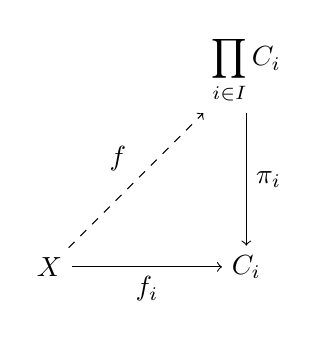
\begin{tikzpicture}[node distance=2.5cm, auto]
	\node (P) {$\displaystyle\prod_{i \in I} C_i$};
	\node (Ci) [below of=P] {$C_i$};
	\node (X) [left of=Ci] {$X$};
	\draw[->] (X) to node [swap] {$f_i$} (Ci);
	\draw[->, dashed] (X) to node {$f$} (P);
	\draw[->] (P) to node {$\pi_i$} (Ci);
\end{tikzpicture}
\end{figure}
\end{proposition}
\begin{proof}
Defina a função
	\begin{align*}
	\func{f}{X}{\prod_{i \in I} C_i}{x}{(f_i(x))_{i \in I}}.
	\end{align*}
Para todo $x \in X$ e para todo $i \in I$,
	\begin{equation*}
	\pi_i \circ f(x) = \pi_i (f(x)) = \pi_i ((f_i(x))_{i \in I}) = f_i(x).
	\end{equation*}
Portanto $\pi_i \circ f = f_i$. Isso mostra a existência da $f$. Para a unicidade, seja $\overline{f}: X \to \prod_{i \in I} C_i$ função tal que, para todo $i \in I$, $\pi_i \circ \overline{f} = f_i$. Seja $x \in X$.  Como $\overline{f}(x) \in \prod_{i \in I} C_i$, $\overline{f}(x) = (x_i)_{i \in I}$. Da propriedade comutativa de $\overline{f}$, segue que, para todo $i \in I$,
	\begin{equation*}
	x_i = \pi_i \circ \overline{f}(x) = f_i(x).
	\end{equation*}
Como $f(x) = (f_i(x))_{i \in I}$, isso mostra que $\overline{f}(x) = f(x)$. Portanto $\overline{f} = f$.
\end{proof}



%O axioma da escolha reescrito para famílias é o seguinte. Para toda família não vazia $(C_i)_{i \in I}$ de conjuntos (disjuntos) não vazios, existe uma função (\emph{função escolha}) $E: I \to \bigcup_{i \in I} C_i$ tal que, para todo $i \in I$, $E(i) \in C_i$.

%\begin{proposition}
%	Seja $(C_i)_{i \in I}$ uma família não vazia de conjuntos. Então
%	\begin{equation*}
%	\prod_{i \in I} C_i = \emptyset \qquad \Leftrightarrow \qquad \exists i \in I \quad C_i = \emptyset.
%	\end{equation*}
%\end{proposition}
%\begin{proof}
%	Primeiro, suponhamos que $(C_i)_{i \in I}$ é uma família de conjuntos não vazios. Então, pelo axioma da escolha, existe uma função $E: I \to \bigcup_{i \in I} C_i$ tal que, para todo $i \in I$, $E(i) \in C_i$. Assim, $E \in \prod_{i \in I} C_i$, o que mostra que $\prod_{i \in I} C_i \neq \emptyset$. Reciprocamente, suponhamos que existe alguma $i \in I$ tal que $C_i = \emptyset$. Então, se existisse $c \in \prod_{i \in I} C_i$, seguiria que $c(i) \in C_i = \emptyset$, o que é absurdo. Logo $\prod_{i \in I} C_i = \emptyset$.
%\end{proof}





\section{Coproduto de conjuntos}

\begin{definition}
Seja $(C_i)_{i \in I}$ uma família não vazia de conjuntos. O \emph{coproduto} de $(C_i)_{i \in I}$ é o conjunto
	\begin{equation*}
	\coprod_{i \in I} C_i :=\set{(i,c)}{i \in I \text{\ \ e\ \ } c \in C_i}.
	\end{equation*}
\end{definition}

\begin{definition}
Seja $(C_i)_{i \in I}$ uma família de conjuntos e $i \in I$. A \emph{inclusão canônica} de $C_i$ em $\coprod_{i \in I} C_i$ é a função
	\begin{align*}
	\func{\iota_i}{C_i}{\coprod_{i \in I} C_i}{c}{(i,c)}.
	\end{align*}
\end{definition}

\begin{proposition}[Propriedade Universal]
Sejam $(C_i)_{i \in I}$ uma família de conjuntos, $X$ um conjunto e, para todo $i \in I$, $f_i: C_i \to X$ uma função. Então existe uma única função $f: \coprod_{i \in I} C_i \to X$ tal que, para todo $i \in I$, $f \circ \iota_i = f_i$ (o diagrama comuta).
\begin{figure}
\centering
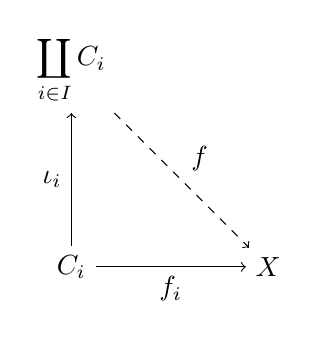
\begin{tikzpicture}[node distance=2.5cm, auto]
	\node (Ci) {$C_i$};
	\node (S) [above of=Ci] {$\displaystyle\coprod_{i \in I} C_i$};
	\node (X) [right of=Ci] {$X$};
	\draw[->] (Ci) to node [swap] {$f_i$} (X);
	\draw[->, dashed] (S) to node {$f$} (X);
	\draw[->] (Ci) to node {$\iota_i$} (S);
\end{tikzpicture}
\end{figure}
\end{proposition}
\begin{proof}
Defina a função
	\begin{align*}
	\func{f}{\coprod_{i \in I} C_i}{X}{(i,c)}{f_i(c)}.
	\end{align*}
Seja $i \in I$ e $c \in C_i$. Então
	\begin{equation*}
	f \circ \iota_i(c) = f(\iota_i(c)) = f(i,c) = f_i(c).
	\end{equation*}
Portanto $f \circ \iota_i = f_i$. Isso mostra a existência da $f$. Para a unicidade, seja $\overline{f}: \coprod_{i \in I} C_i \to X$ função tal que, para todo $i \in I$, $\overline{f} \circ \iota_i = f_i$. Seja $x \in \coprod_{i \in I} C_i$. Existem $i \in I$ e $c \in C_i$ tais que $x=(i,c)$. Da propriedade comutativa de $\overline{f}$, segue que
	\begin{equation*}
	\overline{f}(x) = \overline{f}(i,c) = \overline{f}(\iota_i(x)) = \overline{f} \circ \iota_i(c) = f_i(c) = f(i,c) = f(x).
	\end{equation*}
Isso mostra que $\overline{f}=f$.
\end{proof}


%\cleardoublepage
%\begin{figure}
%\centering
%\begin{tikzpicture}[node distance=4cm, auto]
%	\node (P) {$\displaystyle\prod_{i \in I} C_i$};
%	\node (Ci) [below of=P] {$C_i$};
%	\node (X) [left of=Ci] {$X$};
%	\node (S) [below of=Ci] {$\displaystyle\coprod_{i \in I} C_i$};
%	\node (Y) [right of=Ci] {$Y$};	
%	\draw[->] (X) to node [swap] {$f_i$} (Ci);
%	\draw[->, dashed] (X) to node {$f$} (P);
%	\draw[->] (P) to node {$\pi_i$} (Ci);
%	\draw[->] (Ci) to node {$g_i$} (Y);
%	\draw[->, dashed] (S) to node [swap] {$g$} (Y);
%	\draw[->] (Ci) to node [swap] {$\iota_i$} (S);
%\end{tikzpicture}
%\caption*{Os diagramas comutativos do \\produto e do coproduto de conjuntos.}
%\end{figure}





\cleardoublepage
\subsection{Propriedades de produto e coproduto}

\begin{proposition}
	Seja $(C_{ij})_{(i,j) \in I \times J}$ uma família de conjuntos. Então
	\begin{enumerate}
	\item $\displaystyle \bigcup_{j \in J} \left(\prod_{i \in I} C_{ij}\right) \subseteq \prod_{i \in I} \left(\bigcup_{j \in J} C_{ij}\right)$;
	\item $\displaystyle \bigcap_{j \in J} \left(\prod_{i \in I} C_{ij}\right) = \prod_{i \in I} \left(\bigcap_{j \in J} C_{ij}\right)$.
	\end{enumerate}
\end{proposition}
\begin{proof}
	\begin{enumerate}	
	\item \begin{align*}
	\displaystyle c \in  \bigcup_{j \in J} \left(\prod_{i \in I} C_{ij}\right)
		& \entao \exists j \in J \left(c \in \prod_{i \in I} C_{ij} \right) \\
		& \entao \exists j \in J \ \forall i \in I \left(c_i \in C_{ij} \right) \\
		& \entao \forall i \in I \left(c \in \bigcup_{j \in J} C_{ij} \right) \\
		& \entao  c \in \prod_{i \in I} \left(\bigcup_{j \in J} C_{ij}\right).
	\end{align*}
	
	\item 	
	\begin{align*}
	c \in \displaystyle \bigcap_{j \in J} \left(\prod_{i \in I} C_{ij}\right)
		& \sse \forall j \in J \left(c \in \prod_{i \in I} C_{ij} \right) \\
		& \sse \forall j \in J \ \forall i \in I \left(c_i \in C_{ij} \right) \\
		& \sse \forall i \in I \ \forall j \in J \left(c_i \in C_{ij} \right) \\
		& \sse \forall i \in I \left(c_i \in \bigcup_{j \in J} C_{ij} \right) \\
		& \sse  c \in \prod_{i \in I} \left(\bigcap_{j \in J} C_{ij}\right).
	\end{align*}
	\end{enumerate}
\end{proof}

Notemos que a inclusão contrária no primeiro item nao vale. Suponhamos que para um $j_0 \in J$, todos os $C_{ij_0}$ são vazios, mas para todos outros $j \in J$, os $C_{ij}$ não são vazios. Então o produto desses $C_{ij}$ será sempre vazio, pois sempre tem um dos elementos do produto vazio, e então a união desses produtos será vazia; no entanto, a união desses $C_{ij}$ não será nenhuma vazia e, então, o produto não seráa vazio (pelo axioma da escolha).

\begin{proposition}
\label{conj:proposition.im.inv.prod}
Sejam $X$ um conjunto, $(Y_i)_{i \in I}$ uma família de conjuntos, $(S_i)_{i \in I}$ uma família de subconjutos de $(Y_i)_{i \in I}$, $f: X \to \prod_{i \in I} Y_i$ uma função e, para todo $i \in I$, $f_i := \pi_i \circ f$. Então
	\begin{equation*}
	f\inv\left( \prod_{i \in I} {S_i} \right) = \bigcap_{i \in I} f_i\inv (S_i).
	\end{equation*}
\end{proposition}
\begin{proof}
Note que $x \in f\inv(\prod_{i \in I} {S_i})$ é equivalente a $f(x) \in \prod_{i \in I} {S_i}$, que por sua vez ocorre se, e somente se, para todo $i \in I$, $\pi_i(f(x)) \in S_i$. Como $f_i(x)=\pi_i(f(x)) \in S_i$, isso é equivalente a, para todo $i \in I$, $x \in f_i\inv (S_i)$.
\end{proof}





%\begin{definition}
%Seja $C$ um conjunto não vazio. A \emph{soma} de $C$ é o conjunto
%	\begin{equation*}
%	\coprod C := \set{(X,x) \in C \times \bigcup C}{x \in X}.
%	\end{equation*}
%\end{definition}

%Vale notar que a soma de $C$ existe porque é um subconjunto de $\p\left(C \times \bigcup C \right)$, logo é um conjunto pelo axioma da especificação.

%Definimos a seguir uma nova operação em uma família $(C_i)_{i \in I}$, a soma, também chamada de união disjunta. Em vez de unirmos todos elementos de $(C_i)_{i \in I}$, indexamos cada um deles com o índice do conjunto da família a que ele pertence para que, se um mesmo elemento, digamos $c$, pertencer $C_{i_1}$ e $C_{i_2}$, $i_1,i_2 \in I$ distintos, então na união disjunta $(c,i_1)$ e $(c,i_2)$ serão elementos distintos, enquanto que na união não haverá distinção.



%\begin{conjectura}
%	Seja $(C_i)_{i \in I}$ uma família não vazia de conjuntos. Então
%	\begin{equation*}
%	\coprod_{i \in I} C_i = \emptyset \qquad \Leftrightarrow \qquad \forall i \in I \quad C_i = \emptyset.
%	\end{equation*}
%\end{conjectura}


\subsubsection*{Notação alternativa}

\begin{equation*}
\prod_{i \in I} C_i = \set{\lceil c_i \rceil_{i \in I}}{\forall i \in I \; c_i \in C_i}
\end{equation*}

$\lceil c_i \rceil_{i \in I} = c: I \to \bigcup_{i \in I} C_i$

\begin{equation*}
\coprod_{i \in I} C_i = \set{\lfloor c \rfloor_i}{i \in I, c \in C_i}
\end{equation*}

$\lfloor c \rfloor_i = (i,c)$




\section{Complementares e diferença simétrica}

\begin{definition}
Sejam $X$ e $Y$ conjuntos. O \emph{complementar relativo} de $Y$ em $X$ é o conjunto
	\begin{equation*}
	X \setminus Y := \set{x \in X}{x \notin Y}.
	\end{equation*}
\end{definition}

\begin{definition}
Sejam $X$ um conjunto e $S$ um subconjunto de $X$. O \emph{complementar} de $S$ em $X$ é o conjunto
	\begin{equation*}
	S^\complement := X \setminus S.
	\end{equation*}
%Seja $\mathcal A \subseteq \p(A)$. O \emph{conjunto complementar} de $\mathcal A$ em $A$ é o conjunto
%	\begin{equation*}
%	\complementlement(\mathcal A) := \{X^\complement : X \in \mathcal A\}.
%	\end{equation*}
\end{definition}

\begin{definition}
Sejam $X$ e $Y$ conjuntos. A \emph{diferença simétrica} de $X$ e $Y$ é o conjunto
	\begin{equation*}
	X \difsim Y := (X \setminus Y) \cup (Y \setminus X).
	\end{equation*}
\end{definition}

\subsection{Propriedades}

\begin{proposition}
Sejam $X$, $Y$ subconjuntos de $U$. Então
	\begin{enumerate}
	\item $(X^\complement)^\complement = X$;
	\item $\emptyset^\complement = U$ e $U^\complement = \emptyset$;
	\item $X \cap X^\complement = \emptyset$ e $X \cup X^\complement = U$;
	\item $X \subseteq Y \sse Y^\complement \subseteq X^\complement$.
	\item $(X \cup Y)^\complement = X^\complement \cap Y^\complement$ e $(X \cap Y)^\complement = X^\complement \cup Y^\complement$.
	\end{enumerate}
\end{proposition}




\section{Coberturas e partições}

\begin{definition}
Seja $X$ um conjunto. Uma \emph{cobertura} de $X$ é uma família $(C_i)_{i \in I}$ de subconjuntos de $X$ cuja união é $X$:
	\begin{equation*}
	\bigcup_{i \in I} C_i = X.
	\end{equation*}
Um \emph{subcobertura} de uma cobertura $(C_i)_{i \in I}$ de $X$ é uma cobertura $(C_i)_{i \in J}$ de $X$, com $J \subseteq I$.
\end{definition}

\begin{definition}
Seja $X$ um conjunto. Uma \emph{partição} de $X$ é um conjunto $\mathcal P \subseteq \p(X)$ de subconjuntos de $X$ que satisfaz
	\begin{enumerate}
	\item $\emptyset \notin \mathcal P$;
	\item $\displaystyle\bigcup \mathcal P = X$;
	\item Para todos conjuntos distintos $C_0,C_1 \in \mathcal P$, $C_0 \cap C_1 = \emptyset$.
	\end{enumerate}
Os conjuntos $C \in \mathcal P$ são as \emph{células} de $\mathcal P$.
\end{definition}

Uma partição, se identidicamos um subconjunto de $\p(X)$ com uma família de sunconjuntos de $X$, é uma cobertura de $X$ por conjuntos disjuntos (logo distintos) que não contém o conjunto vazio.

\subsection{Refinamento de partições}

\begin{definition}
Sejam $X$ um conjunto e $\mathcal P$ uma partição de $X$. Um \emph{refinamento} (\emph{superpartição}) de $\mathcal P$ é uma partição $\mathcal R$ de $X$ que satisfaz: para toda célula $D \in \mathcal R$, existe uma célula $C \in \mathcal P$ tal que $D \subseteq C$. Denota-se $\mathcal P \leq \mathcal R$. Diz que $\mathcal P$ é um \emph{engrossamento} (\emph{subpartição}) de $\mathcal R$.
\end{definition}

\begin{proposition}
Sejam $X$ um conjunto e $\mathcal P,\mathcal R$ partições de $X$ tais que $\mathcal P \leq \mathcal R$. Então
	\begin{enumerate}
	\item $\card{\mathcal P} \leq \card{\mathcal R}$;
	\item Para cada célula $C \in \mathcal P$, o conjunto
		\begin{equation*}
		\mathcal R|_C := \set{D \in \mathcal R}{D \subseteq C}
		\end{equation*}
é uma partição de $C$.
	\end{enumerate}
\end{proposition}
\begin{proof}
	\begin{enumerate}
	\item Por definição de refinamento, para toda célula $D \in \mathcal R$ existe célula $C \in \mathcal P$ tal que $D \subseteq C$. Notemos que essa célula $C$ é única pois, se existir célula $C' \in \mathcal P$ tal que $D \subseteq C'$, então $D \subseteq C \cap C'$ e, como $D \neq \emptyset$, segue que $C =C'$. Assim, consideramos a função que mapeia, para cada célula $D \in \mathcal R$ a célula $C_D \in \mathcal P$ tal que $D \subseteq C_D$:
	\begin{align*}
	\func{f}{\mathcal R}{\mathcal P}{D}{C_D}.
	\end{align*}
Mostremos que essa função é sobrejetiva. Para isso, seja $C \in \mathcal P$. Como $\bigcup \mathcal R = X$, para todo $x \in C \subseteq X$ existe $D \in \mathcal R$ tal que $x \in D$. Como $C \neq \emptyset$, existe $x \in C$, logo existe $D \in \mathcal R$ tal que $x \in D$. Por definição de refinamento, existe $C' \in \mathcal P$ tal que $D \subseteq C'$, o que implica $x \in C'$. Como $x \in C' \cap C$, segue que $C=C'$, e concluímos que $D \subseteq C$. Isso mostra que $f(D)=C$, logo que $f$ é sobrejetiva. Concluímos, então, que $\card{\mathcal P} \leq \card{\mathcal R}$.
	
	\item As propriedades 1 e 3 são evidentes por que $\mathcal R$ é partição. Para a propriedade 2, seja $C \in \mathcal P$ e $U := \bigcup \set{D \in \mathcal R}{D \subseteq C}$. Notemos que $C=U$. Para mostrar isso, seja $x \in C$. Então existe $D \in \mathcal R$ tal que $x \in D$, pois $\bigcup \mathcal P=X$. Por definição de refinamento, existe $C' \in \mathcal P$ tal que $D \subseteq C'$, portanto $x \in C'$. Como $x \in C' \cap C$, segue que $C=C'$. concluímos que $D \subseteq C$, portanto que $x \in U$, o que mostra $C \subseteq U$. Reciprocamente, para todo $D \in U$, $D \subseteq C$, portanto $U \subseteq C$, e concluímos que $C=U$.
	\end{enumerate}
\end{proof}

\begin{proposition}
Sejam $X$ um conjunto. A relação de refinamento $\leq$ no conjunto de partições de $X$ é uma relação de ordem parcial.
\end{proposition}

\begin{definition}
Sejam $X$ um conjunto e $(\mathcal P_i)_{i \in I}$ uma família de partições de $X$. O \emph{refinamento comum} a $(\mathcal P_i)_{i \in I}$ é o conjunto
	\begin{equation*}
	\bigvee_{i \in I} \mathcal P_i := \set{\bigcap_{i \in I} C_i}{i \in I,\  C_i \in \mathcal P_i \text{\ \ e\ \ } \bigcap_{i \in I} C_i \neq \emptyset}.
	\end{equation*}
\end{definition}

\begin{proposition}
Sejam $X$ um conjunto e $(\mathcal P_i){i \in I}$ uma família de partições de $X$. O refinamento comum $\bigvee_{i \in I} \mathcal P_i$ a $(\mathcal P_i)_{i \in I}$ é a menor partição de que $X$ que refina $\mathcal P_i$ para todo $i \in I$.
\end{proposition}
\begin{proof}
Primeiro, mostremos que $\mathcal P := \bigvee_{i \in I} \mathcal P_i$ é uma partição. Por definição, $\emptyset \notin \mathcal P$. Seja $x \in X$. Então, para cada $i \in I$, existe $C_i \in \mathcal P_i$ tal que $x \in C_i$, pois $\bigcup \mathcal P_i = X$. Sendo assim, $x \in \bigcap_{i \in I} C_i$, portanto $X \subseteq \bigcup \mathcal P$, e segue que $\bigcup \mathcal P = X$. Por fim, sejam $C=\bigcap_{i \in I} C_i, D=\bigcap_{i \in I} D_i \in \mathcal P$. Se $C \neq D$, então existe $x \in C\setminus D$ ou existe $x \in D \setminus C$. Sem perda de generalidade, suponha o primeiro. Então, existe $i \in I$ tal que $x \notin D_i$. Como $x \in C$, então $x \in C_i$, portanto $C_i \neq D_i$. Mas então, como $\mathcal P_i$ é partição, $C_i \cap D_i = \emptyset$. Por fim, como $C \subseteq C_i$ e $D \subseteq D_i$, segue que $C \cap D = \emptyset$.

Agora mostraremos que $\mathcal P$ é refinamento de $\mathcal P_i$ para todo $i \in I$. Sejam $i \in I$ e $C \in \mathcal P$. Então $\mathcal P=\bigcap_{i \in I} C_i$, portanto $C_i \in \mathcal P_i$. Por fim, sejam $\mathcal R$ partição de $X$ que é refina $\mathcal P_i$ para todo $i \in I$ e $D \in \mathcal R$ uma célula. Então, para todo $i \in I$, existe $C_i \in \mathcal P_i$ tal que $D \subseteq C_i$. Portanto $D \subseteq \bigcap_{i \in I} C_i$, e como $\bigcap_{i \in I} C_i \in \mathcal P$, segue que $\mathcal P \leq \mathcal R$.
\end{proof}

Alguns tipos especiais de partições são úteis na teoria de intergação de Riemmann. Em $\R^1$, essas partições são chamadas de partições de intervalo, e são representadas como um número finito de pontos em um intervalo. Quando generaliza-se para dimensões maiores, usam-se $n$-retângulos, que são conjuntos em $\R^n$ produtos de $n$ intervalos limitados. Podemos fixar um critério a mais, o de que um $n$-retângulo é produto de intervalos fechados em baixo e abertos em cima. Nesse caso, podemos definir que uma partição cujos elementos são $n$-retângulos é uma \emph{malha}.

Alternativamente, quando temos uma medida, que é o caso de $\R^n$, podemos enfraquecer a restrição de que as células de uma partição são iguais ou disjuntas para a de que são iguais ou \emph{quase disjuntas} \--- a interseção tem medida zero \--- e a restrição de que cobrem para a restrição de que a união da partição é quase total \--- seu complementar tem medida nula \--- e por fim, de que nenhum elemento da partição é quase vazio \--- tem medida nula \--- e definir que isso é uma $\mu$-partição ou \emph{quase partição com respeito a $\mu$}.